\documentclass{article}
\usepackage{graphicx}
\graphicspath{{./images/}}
 \usepackage{hyperref}
\usepackage{lipsum}
\usepackage{fancyhdr}
\pagestyle{fancy}
\lhead{\centering{\Large \textbf{Tushar Patil}}}
\cfoot{}
\renewcommand{\headrulewidth}{0.5pt}
\renewcommand{\footrulewidth}{0.5pt}

\begin{document}
	
	\begin{minipage}{2in}
	H.No: 918
	\end{minipage}
	\hfill
	\begin{minipage}{2.25in}
	Contact: 8867514363
	\end{minipage}

	
	\begin{minipage}{2in}
	Sambhaji Nagar,
	\end{minipage}
	\hfill
	Email-id:patil.tushar1998@gmail.com
	
	\begin{minipage}{2in}
	Macche, Belgavi
	\end{minipage}
	
	\begin{minipage}{2in}
	Belgavi - 590014
	\end{minipage}

	\begin{minipage}{2in}
	Karnataka
	\end{minipage}

	\begin{figure}[h!]
		\hfill
		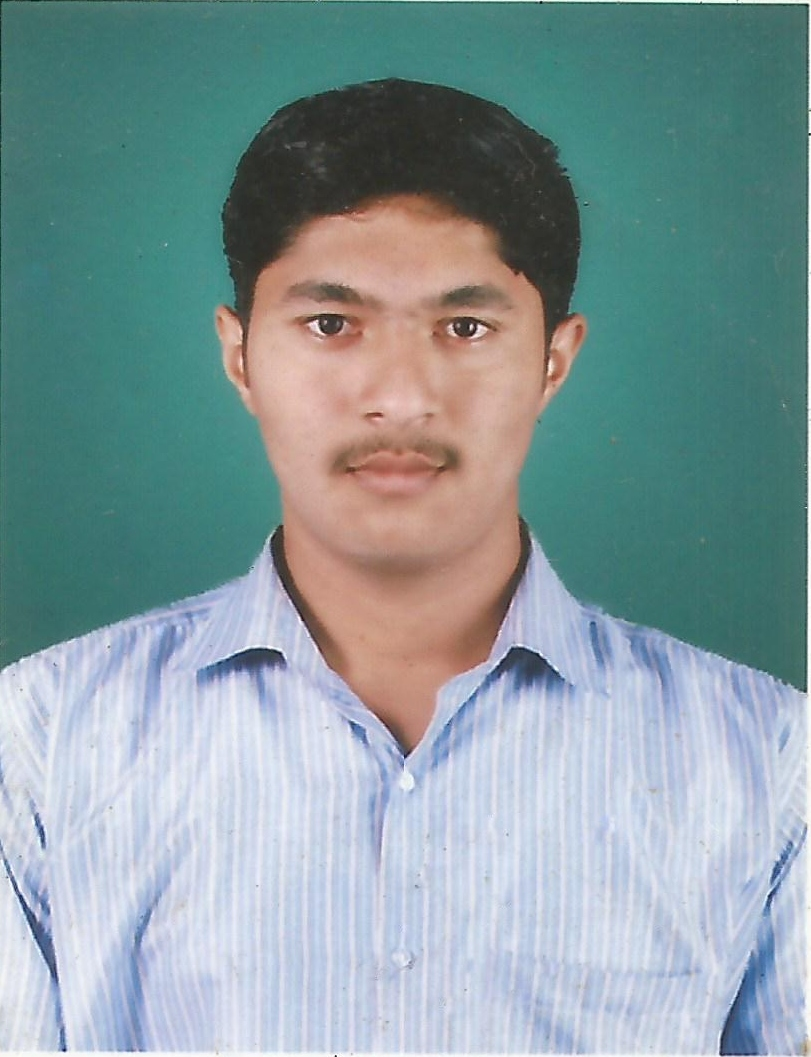
\includegraphics[scale = 0.6]{profilepic.jpg}
		\label{image_1} % Label is used for referencing
	\end{figure}
	
		
\large \textbf{OBJECTIVE:}
	\texttt{	
	To use Computer Science training in Software Development for designing and implementing Applications in various platforms to solve various problems}.\\
\vspace{\baselineskip}
	
	\large \textbf{EDUCATION}:
	
	\begin{tabular}{|c|c|c|c|c|}
	\small Degree & \small College/School & \small University & \small Passing Year & \small Pass Percentage \\
		\hline
		\footnotesize  B.E.(CSE)  & \footnotesize Jain College of Engineering & \footnotesize Visvesvaraya Technological University & \footnotesize 2020 & \footnotesize 7.56(till 5th Sem) \\
		\footnotesize PUC(Science) & \footnotesize MGV-PU College & \footnotesize Karnataka PU Board & \footnotesize 2016 &\footnotesize 74\%  \\
		\footnotesize SSLC & \footnotesize Dnyan Prabodhan Mandir & \footnotesize ICSE & \footnotesize 2014 & \footnotesize 75 \%  \\ 
	
\vspace{\baselineskip}
	\end{tabular}
\\
	\large \textbf{PROJECTS}:\\
	\begin{enumerate}
		\item Blind Calculator | Android App
		\item Online-Quiz | Web Application
		\item Line Following Robot | E-Yantra 2018
		\item Scanner | Android Application\\
		
		\vspace{\baselineskip}
	\end{enumerate}
	\large \textbf{TRAINING \&
		INTERNSHIP:}	
	None\\
	\\
	\large \textbf{RESEARCH PUBLICATIONS :}	
	None\\
	\\
	\large \textbf{TECHNICAL SKILLS
}:
	\begin{itemize}
		\item C
		\item C++
		\item Java
		\item Python
		\item Php
		\item SQL
		\item C\#
		\item HTML \& CSS
		\item JavaScript\\
	\end{itemize}
\large \textbf{SOFT SKILLS:}	
	\begin{enumerate}
	\item Confidence
	\item Listening
	\item Verbal communication
	\item Non-verbal communication
	\item Idea exchange
	\item Curiosity
	\item Self-management
	\item Decision-making
\end{enumerate}

\large \textbf{EXTRA-CURRICULAR ACTIVITIES
:}\\
	\begin{itemize}
	\item Winning 3rd Price in KLE Google IO Extended Competition 2017-2018
	\item Finalist at E-Yantra Competition
\end{itemize}
\large \textbf{CO-CURRICULAR ACTIVITIES
:}\\
	\begin{enumerate}
	\item Department Student Treasurer (FACE)
	\item College Fest Application Development | Android Application
\end{enumerate}

\large \textbf{Personal Details}:\\
Father’s Name: Suhas Patil \\
Mother’s Name: Joshana Patil \\
Sex: Male \\
Date of Birth: 29/08/1998 \\
Nationality: Indian \\
Marital Status: Single \\
\\
\large \textbf{Reference:}\\
\href{Link}{https://github.com/lohitpenu/Internship-eYSIP-2019/blob/master/Latex/Latex-Tutorial-forPresentation.pdf} \\	

\large \textbf{Declaration: }\\
I hereby declare that the information furnished above is true to the best of my knowledge. I do hereby declare that above particulars of information and facts stated are true, correct and complete to the best of my knowledge and belief.\\

\large \textbf{Date: } 17/04/2019\\


\end{document}